\documentclass[a4paper,10pt]{article}
% Use ctrl + alt + V to view live pdf

% Packages
\usepackage[utf8]{inputenc} % For encoding
\usepackage[T1]{fontenc} % Better handling of accented characters and hyphenation
\usepackage{microtype} % Improves spacing and justification
\usepackage{amsmath, amssymb} % For equations and symbols
\usepackage{graphicx} % For including graphics/images
\usepackage{caption} % For customizing figure and table captions
\usepackage{subcaption} % For subfigures and subcaptions
\usepackage{float} % For fixing figure and table positions
\usepackage{booktabs} % For professional-looking tables
\usepackage{siunitx} % For consistent typesetting of units and numbers
\usepackage[margin=2cm]{geometry} % Adjusts page margins
\usepackage{fancyhdr} % For custom headers and footers
\usepackage{lmodern} % For a professional-looking font (main body font)
\usepackage{titlesec} % For title customization
\usepackage{array} % For custom table formatting
\usepackage[colorlinks=true, linkcolor=black, urlcolor=black]{hyperref} % Colored links without boxes
\usepackage{cleveref} % For improved cross-referencing    
\usepackage{multirow}
\usepackage{enumitem}
\usepackage{listings}
\usepackage{xcolor}
\usepackage{textcomp}
\usepackage{tabularx}
\usepackage{changepage}
\usepackage{tikz}
\usepackage{pdfpages}
\usetikzlibrary{shapes.geometric, arrows}
\newcolumntype{Y}{>{\centering\arraybackslash}X}


\lstdefinestyle{vhdl-style}{
    language=VHDL,
    basicstyle=\ttfamily\footnotesize,
    keywordstyle=\bfseries\color{blue},
    commentstyle=\itshape\color{gray},
    stringstyle=\color{red},
    numbers=left,
    numberstyle=\tiny\color{gray},
    stepnumber=1,
    breaklines=true,
    showstringspaces=false,
    frame=single
}
\lstset{style=vhdl-style}
\lstset{captionpos=b}
\lstset{basicstyle=\ttfamily\scriptsize} 
\renewcommand{\lstlistingname}{Program}

% Custom settings
\pagestyle{fancy}
\fancyhf{}
\fancyhead[L]{\textit{GB3 - Risc-V Processor}} % Header left
\fancyhead[R]{\textit{Will Hewes - wh365}} % Header right 
\fancyfoot[C]{\thepage} % Footer center
\setlength{\headheight}{15pt} % Header height
\setlength{\parindent}{0em} % Indentation for paragraphs
\setlength{\parskip}{0.2em} % Add spacing between paragraphs
\setlength{\abovedisplayskip}{0.5em}
\setlength{\belowdisplayskip}{0.5em}
\setlength{\abovedisplayshortskip}{0.5em}
\setlength{\belowdisplayshortskip}{0.5em}
% \setlist{topsep=0em, partopsep=0em, itemsep=0em, parsep=0em}

\graphicspath{{Images/}}

% \renewcommand{\arraystretch}{1.2}

% Title formatting
\renewcommand{\maketitle}{
    \begin{center}
        \LARGE \textbf{ENGINEERING TRIPOS PART IIA} \\ 
        \vspace{0.5em}
        \Large \textbf{GB3 - Risc-V Processor} \\ 
        \vspace{0.5em}
        \textbf{Second Interim Report} \\
        \large Group 4 - Resource Usage \\
        \vspace{1em}
        \large Will Hewes - wh365 \\ 
        Pembroke College \\ 
        \vspace{0.5em}
    \end{center}
}

\begin{document}
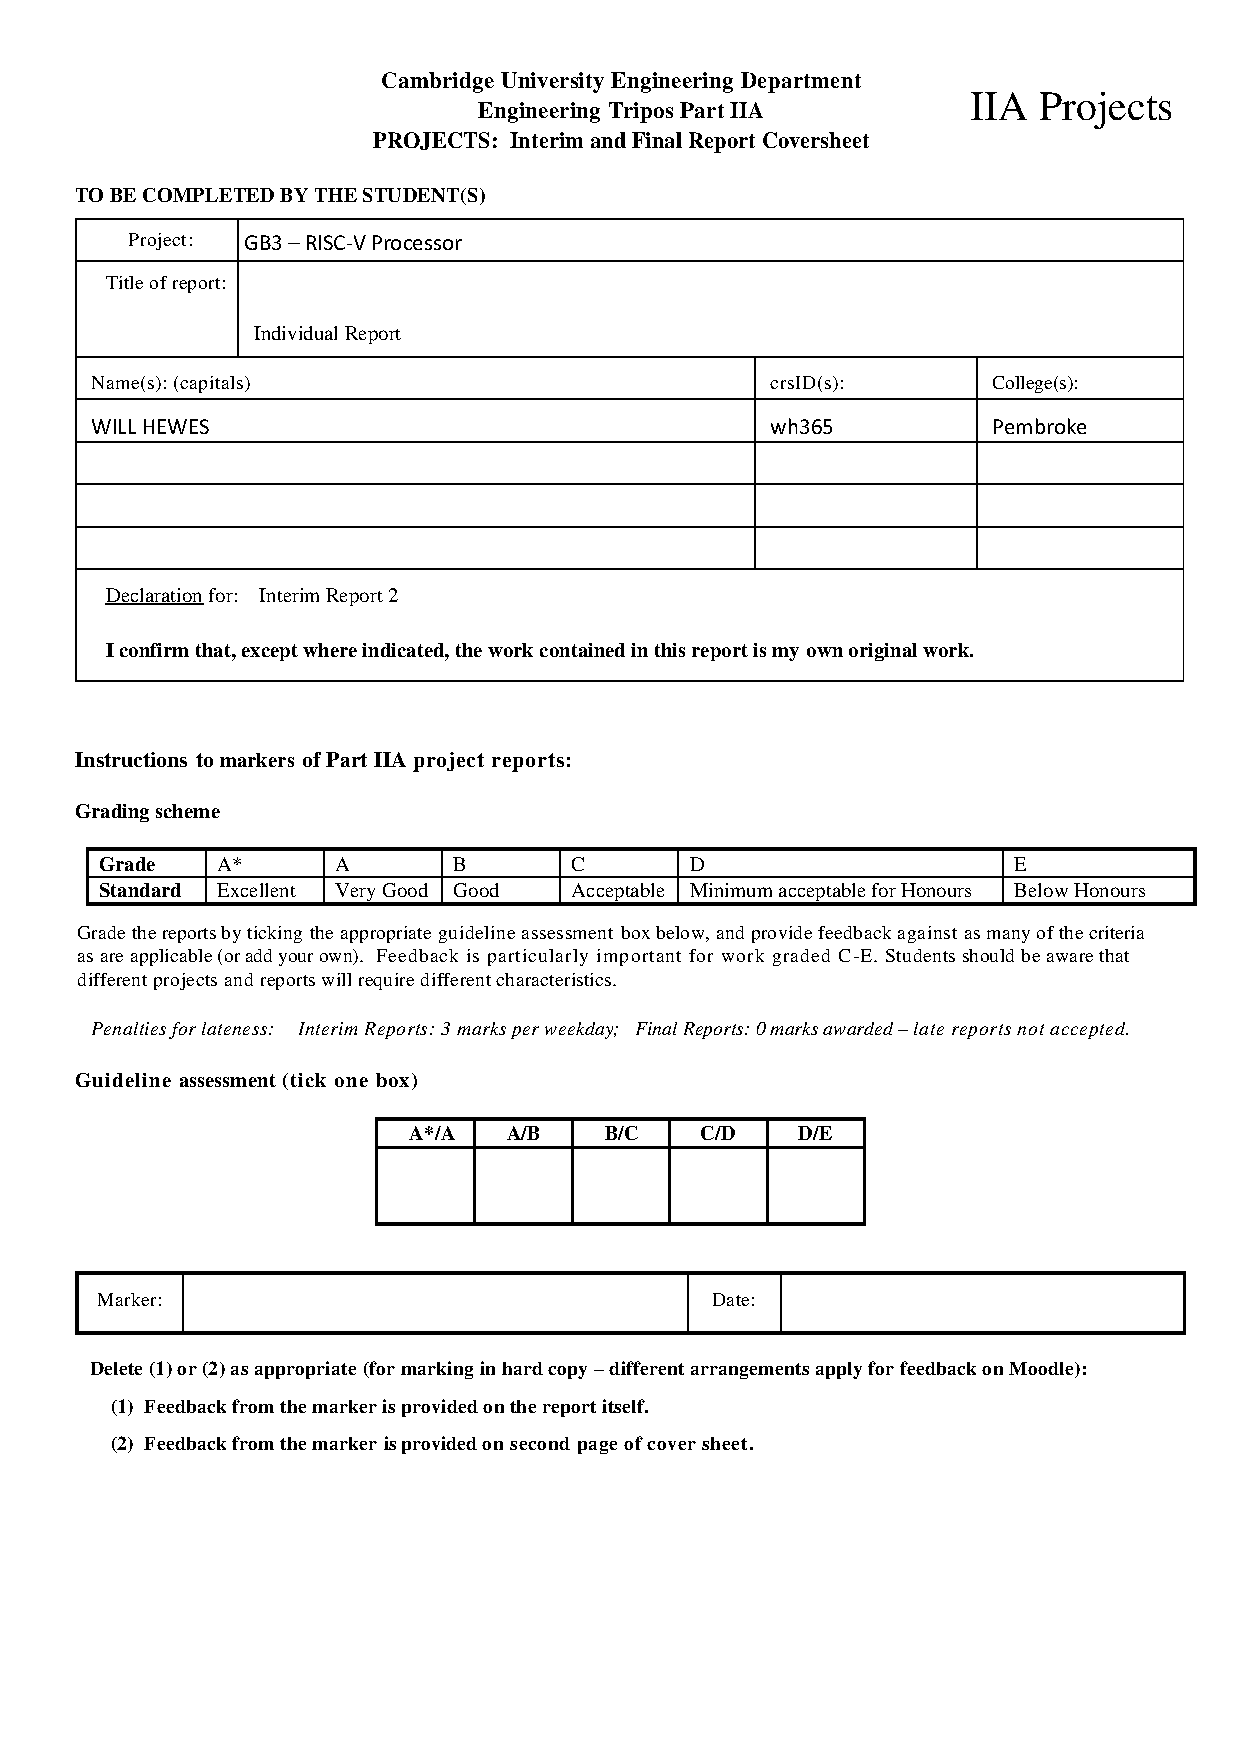
\includepdf[pages=-]{Handouts/IIA Project Coversheet Feedback Interim Report 2.pdf}
\maketitle
\hrule
\tableofcontents
\newpage

\section{Introduction}
\label{sec:Introduction}
% This section should give a detailed introduction to the changes
% you have implemented for your role on the team 
% (power/energy, time, or resource efficiency).

This report covers the changes made to the implementation of the RISC-V processor
with regard to its resource usage. 
The primary aspects that have been targeted for improvement include -


\section{Preliminary Results}
\label{sec:Preliminary_Results}
% This section should provide an detailed quantitative information and results so far.



\section{Potential Risks}
\label{sec:Potential_Risks}
% This section should outline any challenges you ran into, 
% potential risks you see going into the final week, 
% and any steps you are taking to mitigate those risks.

\section{Future Work}
\label{sec:Future_Work}

\section{Conclusion}
\label{sec:Conclusion}

\newpage
\appendix
\label{Appendix}
\section{Resource Usage Data}
%Use this section to include diagrams, Verilog or C code, etc

\end{document}